% Условная компиляция для самостоятельной работы
\ifdefined\mainfile
    % Если это часть основного файла, не добавляем начало и конец документа
\else
    \documentclass[12pt, a4paper]{report}
    \usepackage{/Users/vladbelousov/Desktop/Semestr_4-FP-NSU/Настройка/library}
    \usepackage[utf8]{inputenc} % Подключение поддержки UTF-8
    \begin{document}
\fi

%%-------------------------------%%

\[ I = \frac{ |\vec{E } _1 (\vec{r } ) | ^2 }{2} +\frac{ |\vec{E } _2 (\vec{r } ) | ^2 }{2} +\underbrace{ \mathrm{Re } (\vec{E } _1 (\vec{r } ), \vec{E } _2^{*}  (\vec{r } ))}_{\text{интерференционное слагаемое} } = I_1 + I_2 + I_{12}   \] 

Закон сохранения энергии не нарушается, поскольку интерференция приводит к перераспределения потоков энергии в пространстве. 

Если \( I_{12} = 0  \), то волны не интерферируют, например, в случае \( \vec{E } _1 (\vec{r } )\perp \vec{E } _2 (\vec{r } ) \) - перпендикулярных поляризаций волн. 

Интерференция двух плоских монохроматических волн с эллиптической поляризацией. 

\begin{center}
    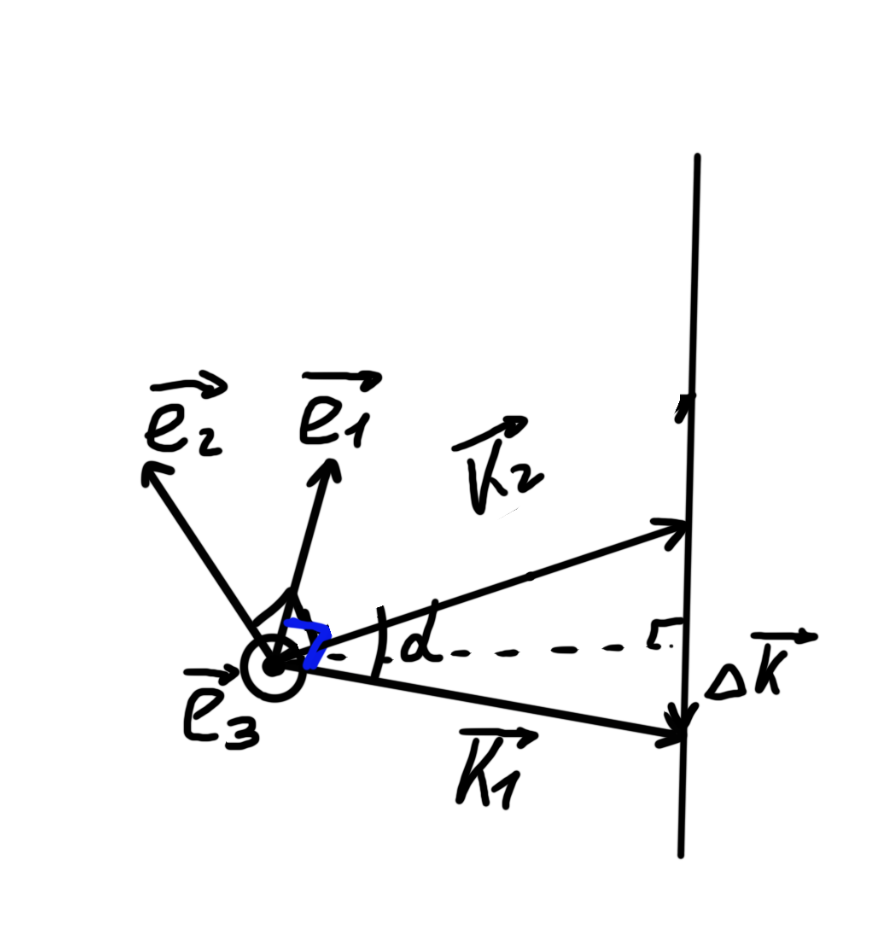
\includegraphics[width=0.4\textwidth]{/Users/vladbelousov/Desktop/Semestr_4-FP-NSU/ЭиО/Лекции_по_дням/image/91.png}
\end{center} 
\[k_1 = \frac{\omega }{c } ,\quad  k_2 = \frac{\omega}{c }   \]
\[ \vec{e } _1 \in  \vec{k}_1 \vec{k } _2 \text{ - плоскости,     } \vec{e}_1 \perp \vec{k } _1    \]  
\[ \vec{e } _2 \in  \vec{k}_1 \vec{k } _2 \text{ - плоскости,     } \vec{e}_2 \perp \vec{k } _2   \]  
\[ \vec{e } _3 \perp   \vec{k}_1 \vec{k } _2 \text{ - плоскости,     } \vec{e}_3 \perp \vec{k } _1 , \text{ } \vec{e}_3 \perp \vec{k } _2   \]  

\[ \vec{E } _ 1 (\vec{r } ) = ( \vec{e } _1 E ^{ ||} + \vec{e } _3 E^{ \perp  }  )e^{ i (\vec{k }_1 , \vec{r } )} , \quad  E_1 ^{||}  , \text{ } E_1 ^{\perp } \in \mathbb{C}    \] 
\[ \vec{E } _2 (\vec{r }  ) = ( \vec{e } _2 E_2 ^{ || }  + \vec{e } _3 E_2^{ \perp }     )e^{ i (\vec{k } _2 ,\vec{r} )}   \] 

\[ I_1 = \frac{(\vec{E }_1 (\vec{r } ) , \vec{E } _1 ^{* } (\vec{r } ) )}{2 } = \frac{1}{2 } [|E _1 ^{||}  | ^2 + |E_1^{\perp } | ^2 ] , \quad  I_2 = \frac{1}{2 }  [|E_2^{||} | ^2 + |E_2 ^{ \perp } | ^2 ]  \] 

\[ I_{12} = \mathrm{Re }  [ ((\vec{e } _1 ,\vec{e } _2 ) E_1^{||}E_2 ^{||*} + E_1^{ \perp } E_2 ^{\perp *}    )e^{i ((\vec{k }_1 - \vec{k } _2  ), \vec{r} )} ]  \] 

\[ E_1 ^{ || }  E_1 ^{ || * } = |E_1 ^{||} ||E_2 ^{||} | e^{ i \varphi_1} = |E_1 ^{||} | e^{ i \mathrm{arg } E_1 ^{||}  } \cdot |E_2 ^{||} |e^{- i \mathrm{arg } E_2^{||}  }  \quad  (\varphi_1 = \mathrm{arg } E_1 ^{ ||}  - \mathrm{arg } E_2 ^{ ||}   )     \] 
\[ E^{ \perp  }E_2^{ \perp * } = |E_1   ^{ \perp } ||E_2 ^{\perp } |e^{ i \varphi_2 } , \quad  I_{12} = (\vec{e } _1 ,\vec{e } _2 ) |E_1 ^{ || } ||E_2 ^{ ||} | \cos ((\Delta \vec{k } , \vec{r } )+ \varphi_1 )+ |E_1 ^{ \perp }  ||E_2 ^{\perp } | \cos    ((\Delta \vec{k } ,\vec{r } )+ \varphi_2  ) \] 

\[ I = I^{ || }  + I ^{ \perp  }  \] 
\[ I ^{ ||    } = \frac{1}{2 }  |E_1 ^{ ||} |  ^2 + \frac{1}{2 }  |E_2 ^{||} | ^2  + (\vec{e } _1 ,\vec{e } _2 ) |E_1 ^{||} ||E_2 ^{ ||} | \cos  ((\Delta \vec{k } , \vec{r } )+ \varphi_1)  \] 
\[ I^{ \perp } = \underbrace{\frac{1}{2 }  |E_1 ^{ \perp} |  ^2 }_{I_1^{\perp } }+ \underbrace{\frac{1}{2 }  |E_2 ^{\perp} |  ^2}_{I_2^{\perp } } +\underbrace{ |E_1 ^{\perp} ||E_2 ^{ \perp} | }_{2 \sqrt{I_1 ^{\perp } I_2^{\perp }  }}\cos  ((\Delta \vec{k } , \vec{r } )+ \varphi_2)  \] 

Пример: \( E_1^{ ||} = E_2 ^{||}  =0    \) 
\[ I^{ \perp } = I_1^{\perp } + I_2 ^{\perp } +2\sqrt{I_1 ^{\perp } I_2 ^{\perp }   } \mathrm{cos}   (\underbrace{(\Delta \vec{k }  ,\vec{r } )}_{\Delta k \cdot x} + \varphi_2)   \] 
\[ \max  I^{\perp } = I_1 ^{\perp } + I_2 ^{\perp  } +2 \sqrt{I_1 ^{\perp }I_2 ^{\perp }  } = (\sqrt{ I_1^{\perp }} +\sqrt{I_2 ^{\perp } }  ) ^2 ,\quad  \min  I^{\perp } = I_1 ^{ \perp } + I_2 ^{\perp } - 2    \sqrt{I_1 ^{\perp }I_2 ^{\perp }  } = ( \sqrt{I_1^{\perp }} -\sqrt{I_2 ^{\perp }}   ) ^2    \] 


\begin{center}
    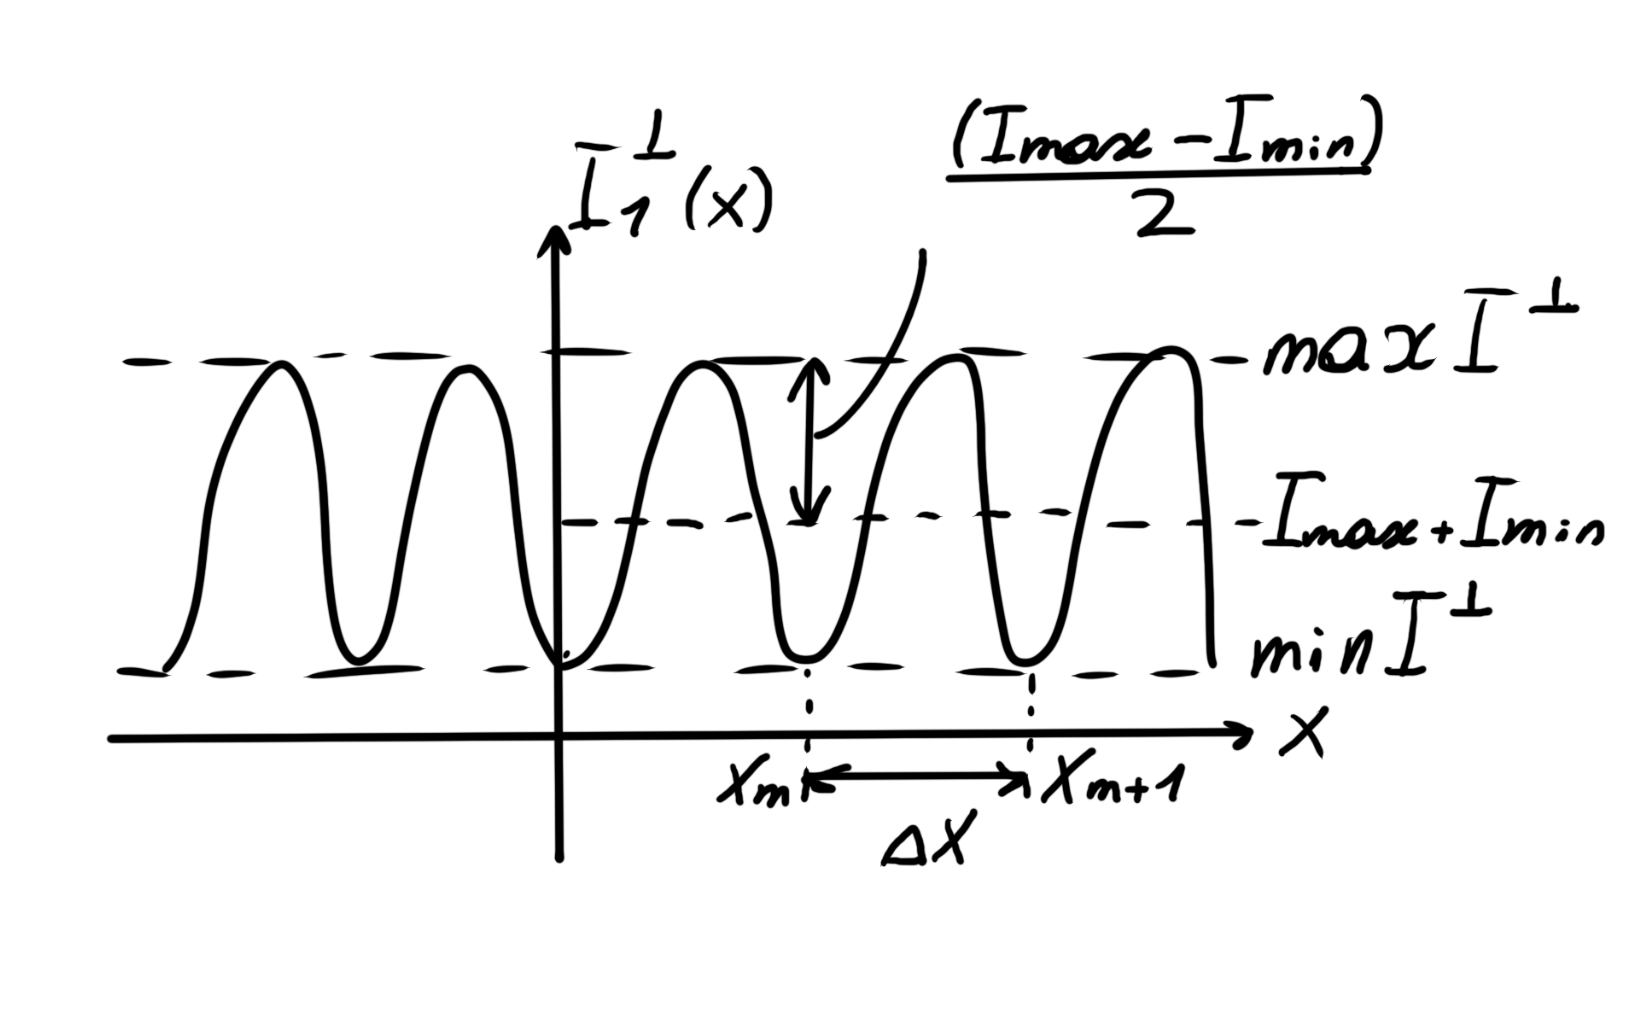
\includegraphics[width=0.55\textwidth]{/Users/vladbelousov/Desktop/Semestr_4-FP-NSU/ЭиО/Лекции_по_дням/image/92.png}
\end{center} 
\[ \Delta x \text{ - период интерференционной картины }  \] 

\[ \Delta x \cdot \Delta k = 2 \pi  \] 

\[ \begin{aligned}
\begin{cases}
    x_m \Delta k = 2 m \pi + \pi    \\
    x_{m+1 }  \Delta k = 2 ( m+1 ) \pi + \pi
\end{cases}
\quad  \Rightarrow \Delta x \cdot \Delta k  = x_{m+1 }  - x_m = 2 \pi 
\end{aligned} \] 

\[ \Delta x = \frac{ 2\pi  }{\Delta k}  =\frac{2 \pi }{2 |\vec{k}_1 |\sin  \frac{\alpha}{2 }} = \frac{\lambda}{2 \sin  \frac{\alpha}{2 } }      \] 
\[ \text{Если } \alpha \ll 1 , \text{ } \Delta x \approx \frac{\lambda}{\alpha } = \frac{ 0, 5 \text{ мкм } }{\alpha } \sim 1 \text{ мм}   \Rightarrow \alpha \sim  10^{- 3 } \text{ рад}  \] 

\textbf{Видность: } \( \displaystyle  V = \frac{ I_{ \max  } - I_{ \min  }  }{ I_{ \max  } + I_{ \min }  }  \) 

Для человеческого глаза \( \min  V  \), при которой видна интерференционная картина, \( = 0,5 \) 

\[ V = \frac{ 4 ( I_1 ^{\perp  }I_2 ^{ \perp }   )}{2 (I_1 ^{\perp  } +I_2 ^{\perp }  )} = \frac{2 ( I_1 ^{\perp } I_2 ^{\perp }  )}{I_1 ^{\perp } + I_2 ^{\perp }  } = \frac{2 \sqrt{\frac{ I_1^{\perp } }{I_2 ^{\perp } } }}{\frac{I_1^{\perp } }{I_2 ^{\perp } } +1}   \] 

\begin{center}
    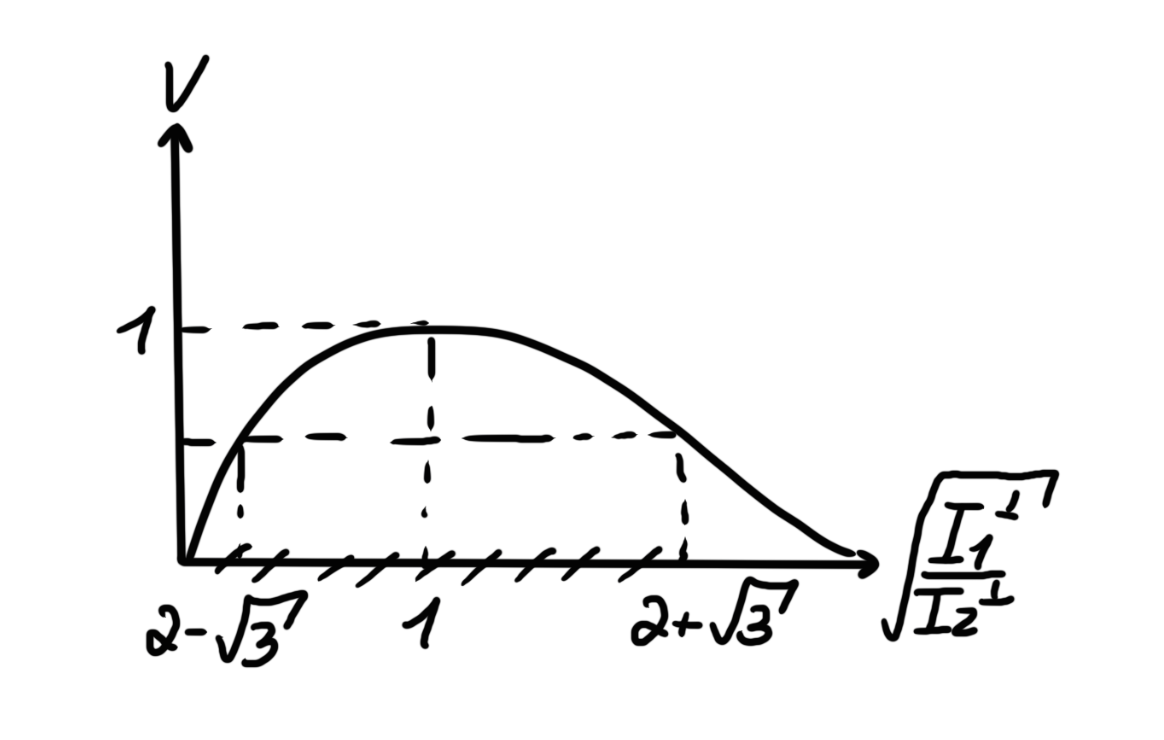
\includegraphics[width=0.55\textwidth]{/Users/vladbelousov/Desktop/Semestr_4-FP-NSU/ЭиО/Лекции_по_дням/image/93.png}
\end{center} 

\section{Интерференция волн двух точечных источников (сферических волн)}

\begin{center}
    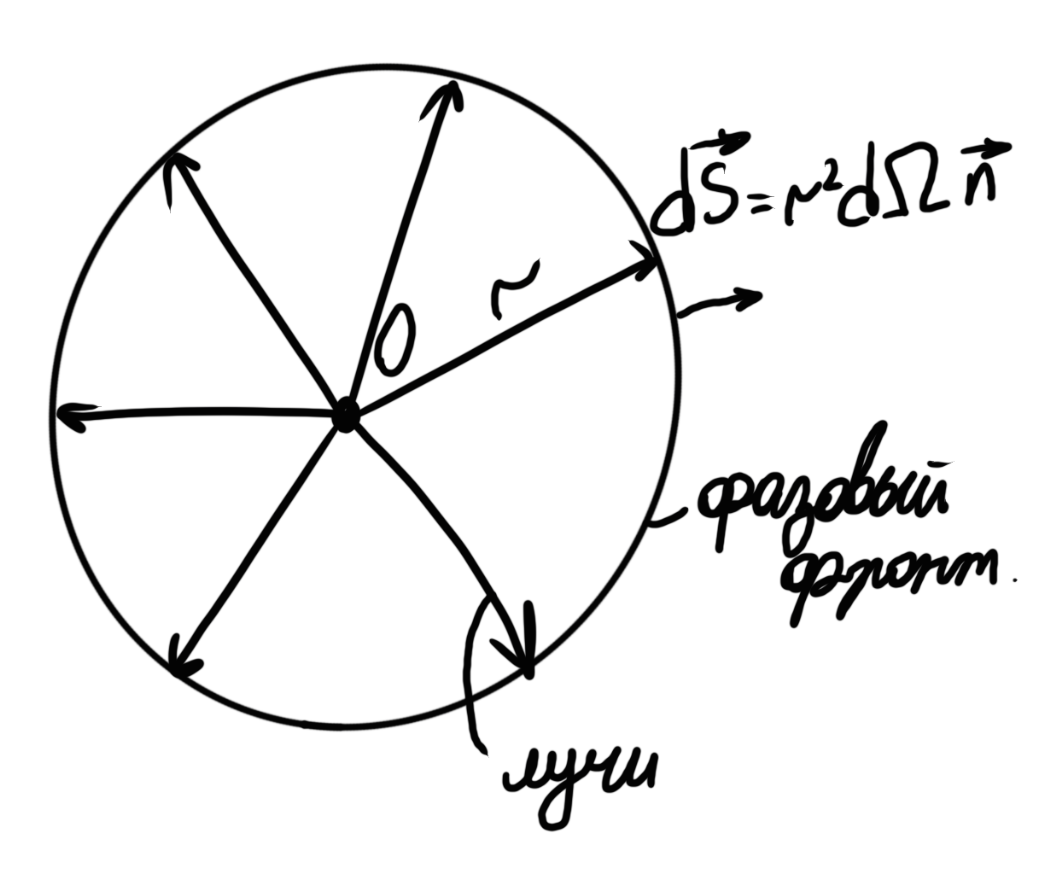
\includegraphics[width=0.4\textwidth]{/Users/vladbelousov/Desktop/Semestr_4-FP-NSU/ЭиО/Лекции_по_дням/image/94.png}
\end{center} 
\[  \psi (\vec{r } )  = \int_{0}^{ r} n ds  = nr  \] 
\[ \vec{E }  (\vec{r },t  )  = \vec{E } _0 \frac{L}{r } e^{ i k_0 \psi (\vec{r }) - i \omega t } = \vec{E } _ 0 \frac{L}{r}  e^{ i k r - i\omega t }   \] 
\[ \vec{B} (\vec{r },t       ) = \vec{B } _0 \frac{L}{r } e^{ i k r - i \omega t }  \] 

\[ <\vec{\mathbb{S} } >  = \frac{c}{8 \pi } \mathrm{Re }  [ \vec{E }  (\vec{r } ) \times  \vec{H } ^{ * } (\vec{r } )]_{\text{Г} }  \sim \frac{A }{r ^2  } \vec{e } _r \Rightarrow \int_{\text{cфера }r  }  (<\vec{\mathbb{S}} > d \vec{s } ) = \int \frac{ A }{r ^2 } r ^2 d \Omega = \mathrm{const}      \] 

\begin{center}
    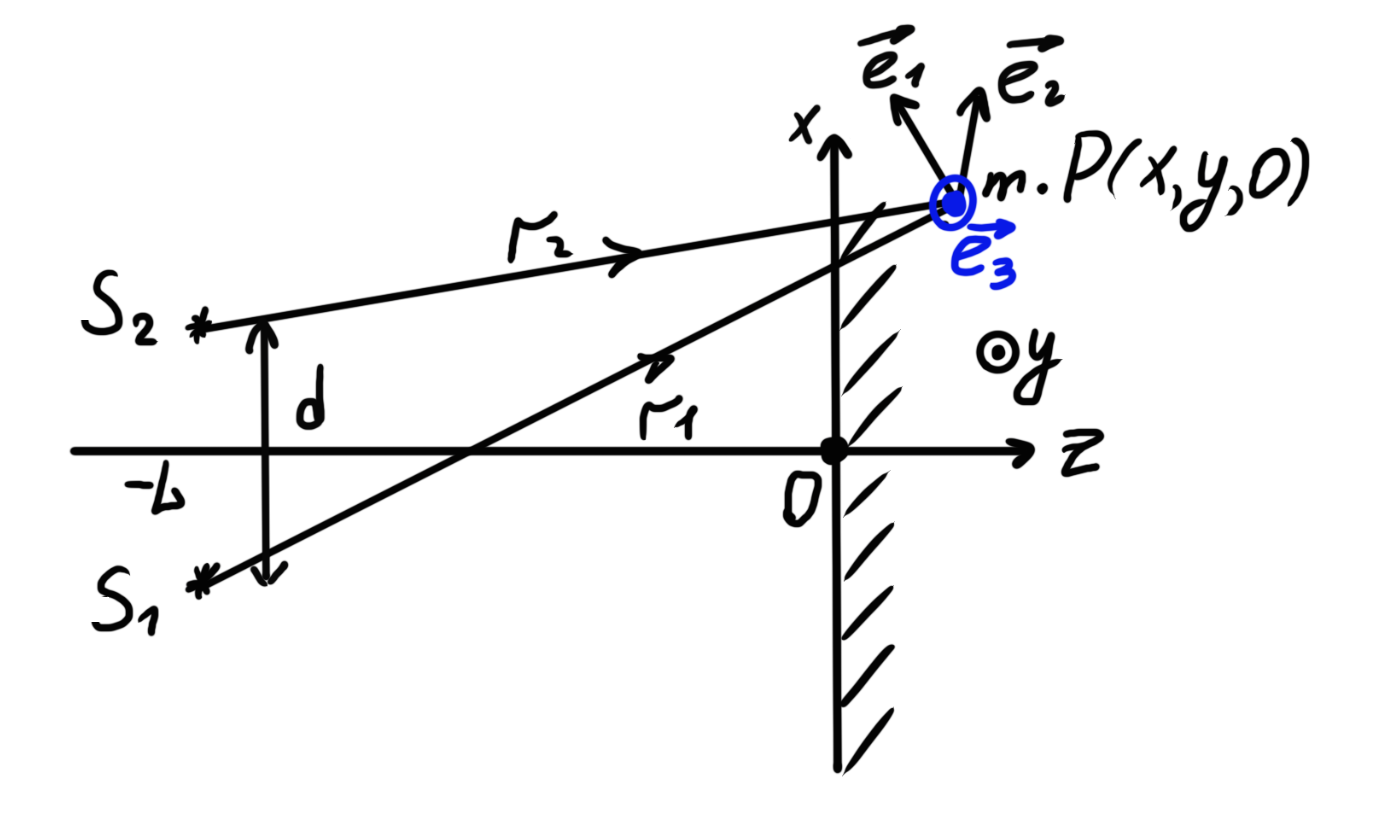
\includegraphics[width=0.55\textwidth]{/Users/vladbelousov/Desktop/Semestr_4-FP-NSU/ЭиО/Лекции_по_дням/image/95.png}
\end{center} 
\[ S_1 \text{ и } S_2 \text{  в плоскости } (x, z )  \] 

\[ \vec{E } _1 (\vec{r }_1   ) \perp  \vec{r }  _1 , \text{ }  \vec{E } _2 (\vec{r } _2 ) \perp  \vec{r } _2  \] 
\[ \vec{E } _1 (\vec{r } _1 ) = \frac{L}{r_1} (E_1 ^{ || }  \vec{e }  _1 + E_1 ^{\perp  } \vec{e } _3  ) e^{ i k r_1 } , \quad  E_1 ^{ || }  ,\text{ }    E_1 ^{ \perp  } \in  \mathbb{C}   \]  
\[ \vec{E } _2 (\vec{r } _2 ) = \frac{L}{r_2} (E_2 ^{ || }  \vec{e }  _2 + E_2 ^{\perp  } \vec{e } _3  ) e^{ i k r_2 } , \quad  E_2 ^{ || }  ,\text{ }    E_2 ^{ \perp  } \in  \mathbb{C}   \]  

\[ I_1  = \frac{1}{2 }  \frac{ L ^2 }{r_1 ^2 } ( |E_1 ^{|| } | ^2 + |E_1 ^{\perp } | ^2 )  \] 
\[ I_2 = \frac{1}{2 }  \frac{ L ^2 }{r_2  ^2 } ( |E_2 ^{ ||} | ^2 + |E_2 ^{\perp }  | ^2 )   \] 

\[ I_{12} = \mathrm{Re }  (\vec{E } _1 (\vec{r}_1 )), \vec{E } _2 ^{ * } (\vec{r}_2 )  = \frac{L ^2 }{r_1 r_2 } \mathrm{ Re } [((\vec{e } _1 , \vec{ e } _2 )E_1 ^{||}  E_2 ^{\perp* } + E_1 ^{\perp } E_2 ^{|| *}) e^{i k r_1 - i k r_2 }   ]  =\]  
\[ = \frac{L ^2 }{r_1 r_2 } [ \cos  \alpha |E_1 ^{||} | |E_2 ^{||} |\cos (\Delta k r + \varphi_1 )+ |E_1 ^{\perp } ||E_2^{\perp } |\cos (\Delta k r + \varphi_2 )]\Rightarrow I = I^{||}  + I^{\perp }   \] 

\[ I^{\perp } = \underbrace{\frac{L ^2}{2r_1 ^2 } |E_1 ^{\perp } | ^2}_{I_1^{\perp } } + \frac{L ^2 }{2 r_2 ^2 }|E_2 ^{\perp } | ^2   + \frac{L ^2 }{r_1 r_2 } |E_1 ^{\perp }  |  |E_2^{\perp } | \cos  (k \Delta r + \varphi_2 ) \] 

\( I_1  \) - интенсивность излучения от \( s_1  \) в точке \( P \) 

\[ I^{\perp } = I_1 ^{\perp } + I_2 ^{\perp } +2 \sqrt{I_1 ^{\perp }I_2 ^{\perp }  } \cos (k \Delta r + \varphi_2 )   \] 

Обычно в интерференционных схемах используют параксиальное приближение \( \Rightarrow x,y, d \ll L \) 

\[ \Delta r = r_1 -r_2 = \frac{ (r_1 - r_2 )(r_1 +r_2 )}{r_1 +r_2 } = \frac{ r_1 ^2 + r_2 ^2 }{r_1 + r_2 } , \quad  r_1 ^2  = \left( x + \frac{d}{2 }  \right) ^2 + y ^2+ L ^2 ,\quad  r_2 ^2 = \left(  x - \frac{d}{2 }  \right) ^2 + y ^2 + L ^2      \] 
\[ \Delta r = \frac{ x d }{\frac{r_1 + r_2 }{2 } }= \frac{xd}{r} \approx \frac{xd}{L}   \] 

\[ I^{\perp } = I_1^{\perp } + I_2 ^{\perp } + 2\sqrt{I_1 ^{\perp }I_2 ^{\perp }  } \cos \left( \frac{kxd}{L } + \varphi_2  \right)    \] 

\begin{center}
    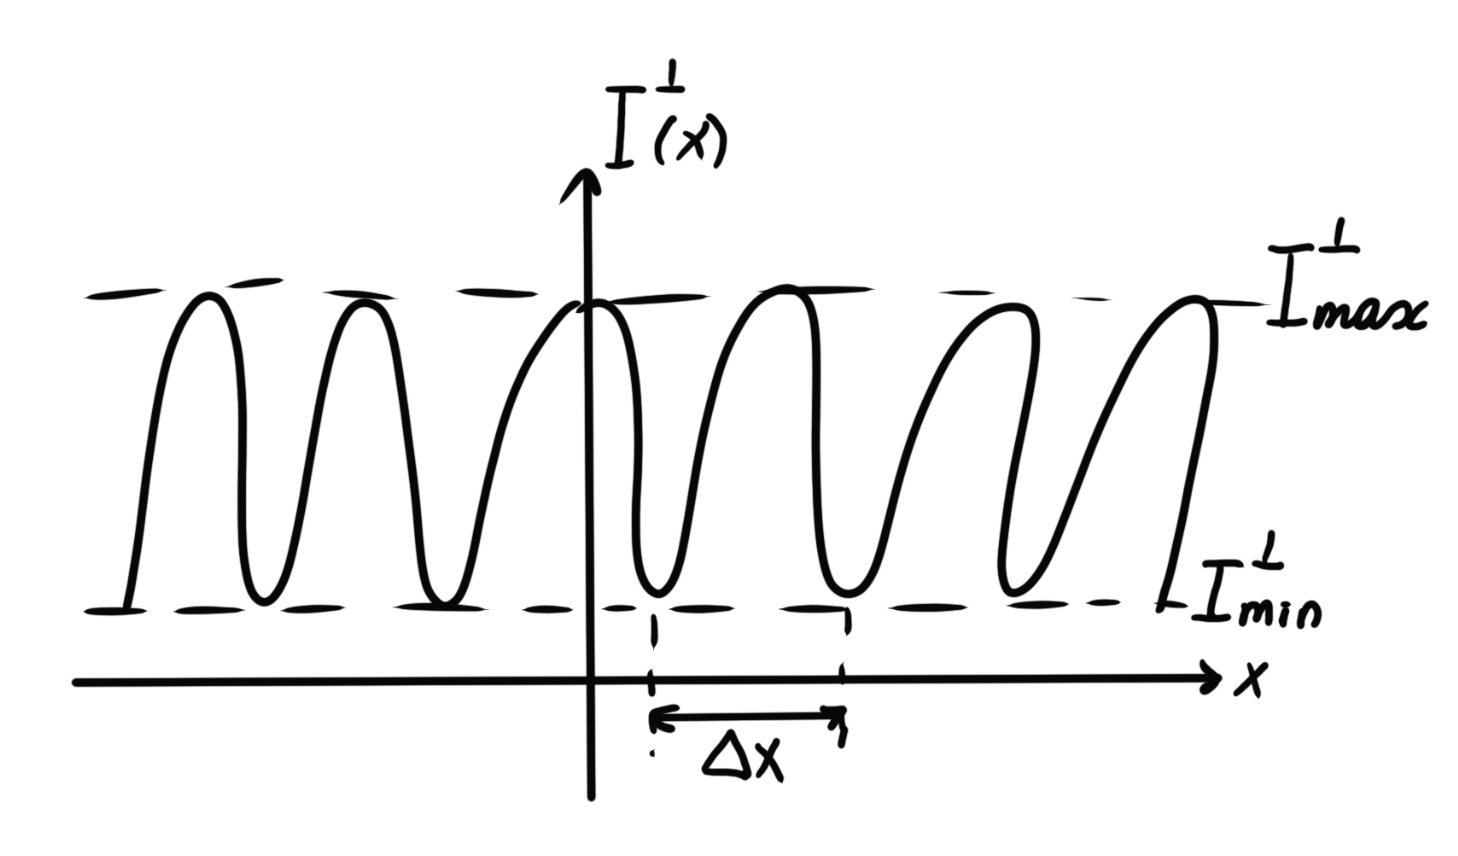
\includegraphics[width=0.55\textwidth]{/Users/vladbelousov/Desktop/Semestr_4-FP-NSU/ЭиО/Лекции_по_дням/image/96.png}
\end{center} 

\[ \frac{k \Delta x d }{ K }  = 2 \pi \Rightarrow \Delta x = \lambda \frac{L}{d}   \] 

\section{Излучение скопления спонтанно излучающихся атомов }

\begin{center}
    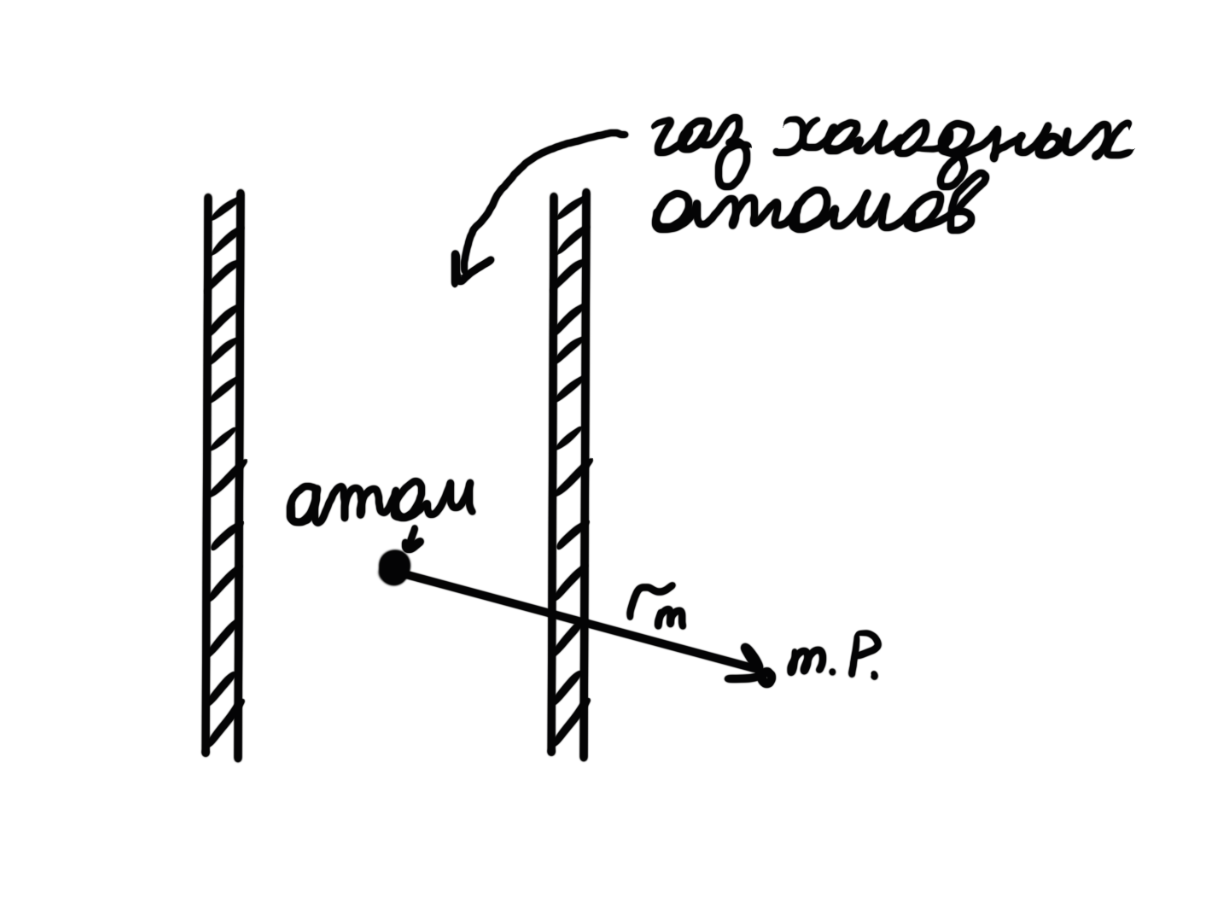
\includegraphics[width=0.55\textwidth]{/Users/vladbelousov/Desktop/Semestr_4-FP-NSU/ЭиО/Лекции_по_дням/image/97.png}
\end{center} 
\[ \vec{E } _a (\vec{r }   ,t ) = \begin{cases}
\displaystyle \vec{E } _0 \frac{L}{r} e^{i k r - i \omega_0 t } e^{- \gamma t } , \text{ }  t> \frac{r}{c}  \\
\displaystyle 0 , \text{ }  t < \frac{r} {c}   
\end{cases} \] 

Если атом начинает излучать в момент \( t_{m_0}       \): 

\[ \vec{E } _{m }  (\vec{r}  _m , t ) = \begin{cases}
\vec{E }_0 \frac{L}{r_m } e^{ - i \omega_0(t - t_m )} e^{- \gamma (t- t_m )} , \text{ } t>t_m\\
0 , \text{ } t<t_m    
\end{cases} \] 
\[ t_m = t_{ m_0} + \frac{ r_m }{c}   \] 

Пусть \( L\gg  \) размер кюветы \(\displaystyle  \Rightarrow \frac{L }{r_m } \approx 1   \)

\[ \text{В точке P: } \vec{E }  _{\Sigma } (t ) = \sum_{m =1} ^{M_0 }\vec{E } _m   = \sum_{m =1}^{M_0 } \vec{E } _0 e^{- i \omega_0 (t -t_m )- \gamma(t - t_m)}      \] 

\begin{center}
    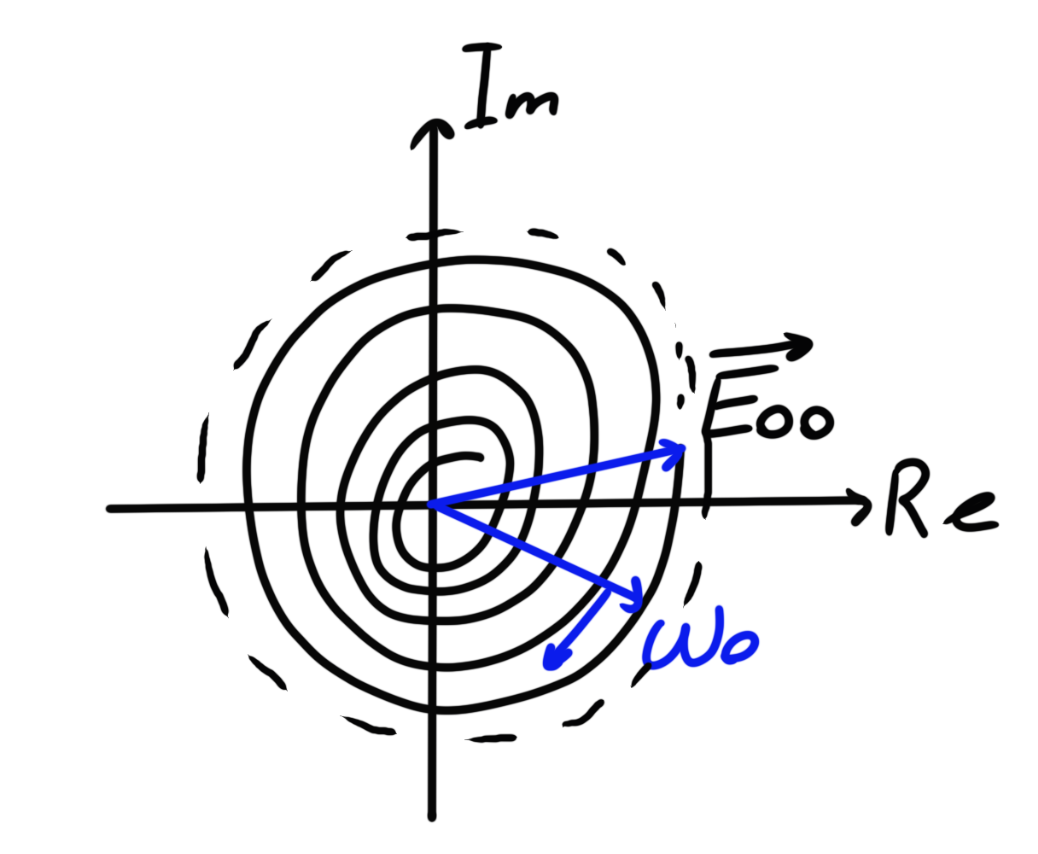
\includegraphics[width=0.4\textwidth]{/Users/vladbelousov/Desktop/Semestr_4-FP-NSU/ЭиО/Лекции_по_дням/image/98.png}
\end{center} 



%%-------------------------------%%

% Закрытие документа, если файл компилируется отдельно
\ifdefined\mainfile
    % Если это основной файл, не нужно заканчивать документ
\else
    \end{document}
\fi

